\subsection{Transfer-to-Population ratio}
While the aggregate Net Transfer is positive for immigrants and negative for natives for 2015, this trend is relatively recent as it became apparent only from 2012.
\autoref{fig:aggTrend} shows that the opposite trend was prevailing till 2001, with immigrants contributing about 5\% more than their population share.
Between 2002 and 2011, immigrants and natives contributed to public finances roughly in the same proportion as their population share.
While the trend in outflows has reversed throughout the study period for the two populations, the trend in inflows has been much stable, especially for natives who received between one and two percent less public transfer than their population share.
For immigrants, the cost was about 10\% more till 2001 but decreased gradually to about 5\% more than their population.

  \begin{figure}[H]%
    \caption{Transfer share as a ratio to Population share for immigrants and natives between 1997 to 2015}
    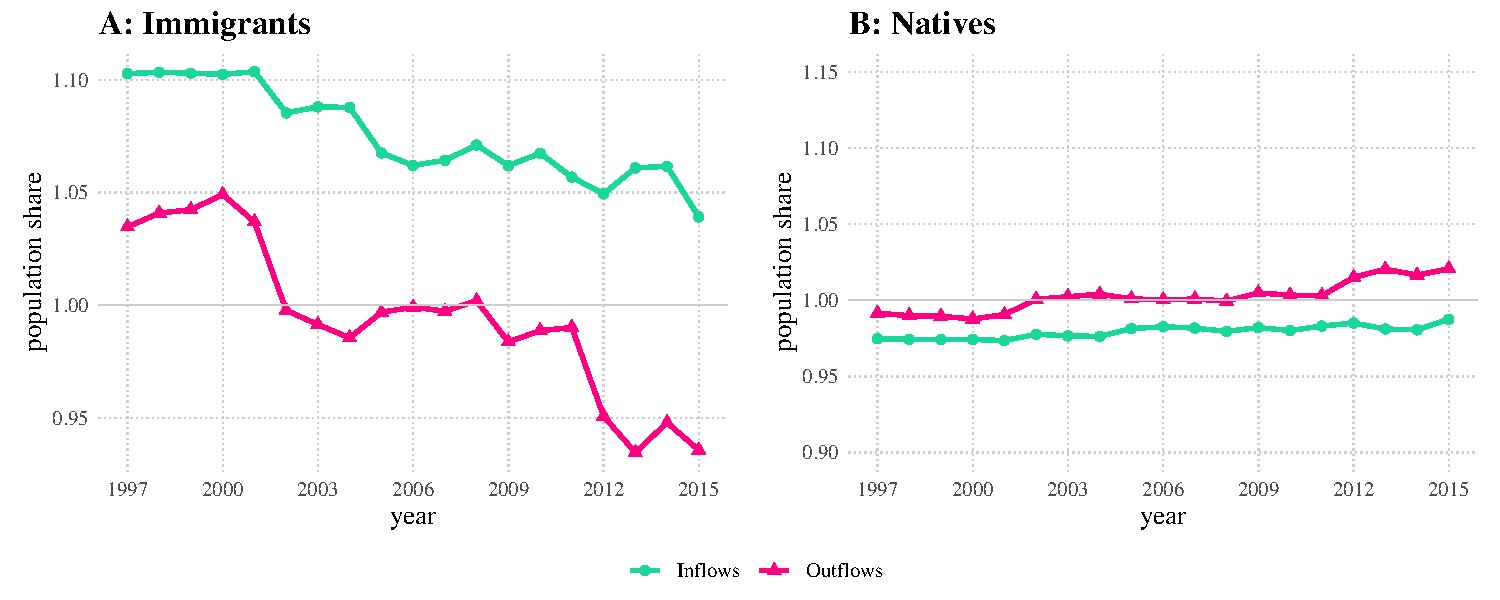
\includegraphics[width=1\textwidth]{../ntaImmig/res/aggTrend.pdf}%
    \label{fig:aggTrend}%
  \end{figure}%

Although aggregate measures provide exciting insights about the relative cost of immigration in Canada, crude per-capita values are better indicators for comparing immigrants and natives, as they remove the effect of the population size. \autoref{fig:netDiff} shows the trends in crude per-capita values for Net Transfers (A) on one hand and Immigrant Surpluses (B) on the other hand between 1997 and 2015.

\subsection{Net Transfer of immigrants and natives}
Excluding the sudden increase from 2011, which increased it to \DTLfetch{statex}{sKey}{AveperCapita}{sVal}\$, the average Net Surplus of transfer has fluctuated only slightly around \$1400 since 1997.
A positive Net Surplus of transfer implies that the average immigrant has cost the state more than the average native.
However, this overall unfavourable cost says little about the origins of these costs, as it hides significant differences in trends within each group and transfer components.

\vspace{0.7em}\par
Looking at the trend in Net Transfer (\autoref{fig:netDiff}-A) separately for immigrants and natives, it can be observed that immigrants have had a positive Net Transfer over the studied period.
This positive Net Transfer implies that immigrants have consistently received more transfers from the state than contributing to its revenues.
Between 1997 and 2011, the average Net Transfer for immigrants fluctuated around \$1400 per year.
However, it rose rapidly between 2011 and 2013 to surpass \$2100.
Although at a much lower level, natives have also seen a positive Net Transfer between 1997 and 2002.
However, Net Transfer among natives has dropped and become negative since 2003.
Between 2005 and 2015, Net Transfer among natives mostly has been negative with slight fluctuation around \$280, a sign that they contribute more to the public purse than they received from it.

  \begin{figure}[H]%
    \caption{Difference in Inflows and Outflows transfers for immigrant and natives between 1997 to 2015}
    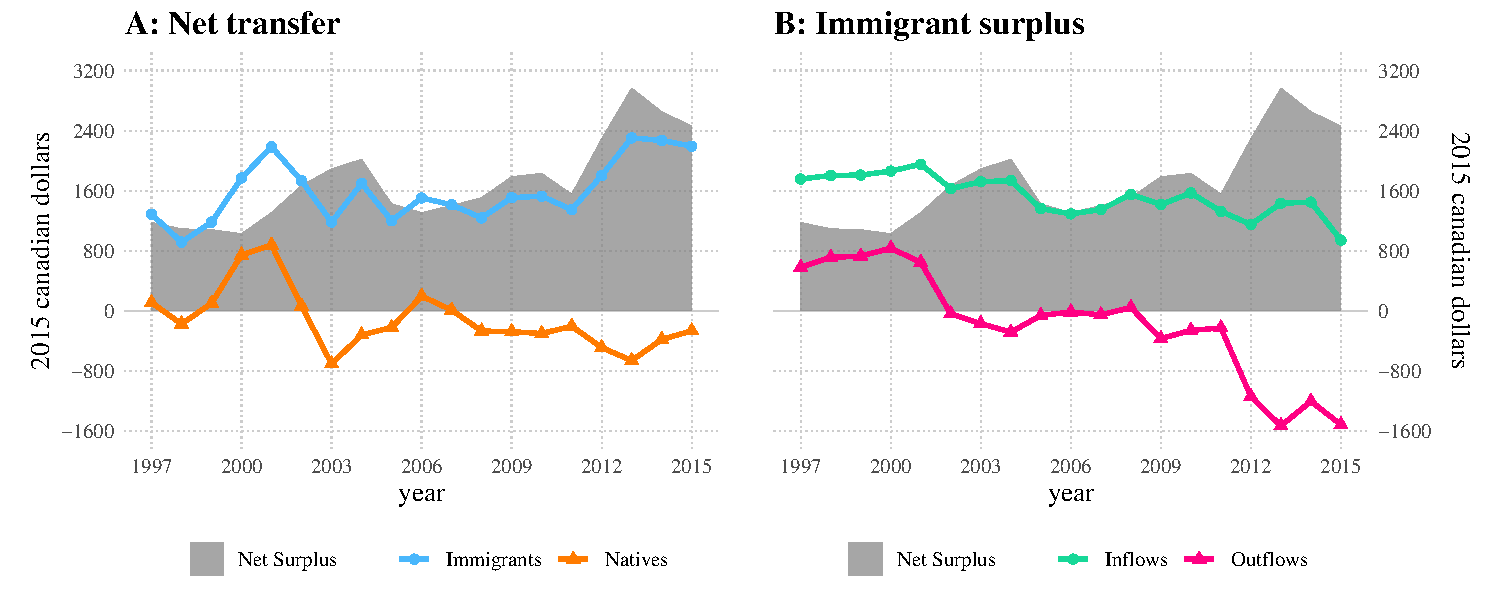
\includegraphics[width=1\textwidth]{../ntaImmig/res/netDiff.pdf}%
    \label{fig:netDiff}%
  \end{figure}%

\vspace{0.7em}\par
Together, these observations suggest that immigrants have consistently received more than they contributed.
In contrast, natives have received slightly less than they contributed, leading to a consistently positive Net Surplus between 1997 and 2011.
However, it is still unclear how surpluses in inflows and outflows have trended during the studied period and which one contributed the most to the sudden increase in the Net Surplus from 2012.
\autoref{fig:netDiff}-B analyze the trend in Immigrant Surplus for inflows and outflows, which may provide further clarification.

\subsection{Immigrant Surplus for Inflows and Outflows}
Over the studied period, the Immigrant Surplus for inflow has been positive, with immigrants receiving about \$\numprint{1400} more than natives on average.
However, the trend is downward, suggesting that transfers to immigrants have been decreasing compared to natives.
For instance, the surplus has dropped by about \$700 between 1997 and 2015 for inflows. Along with this trend, if the surplus for outflows maintained their early 2000s level, the Net Surplus between immigrants and natives would be close to null by 2015.
Instead, while the surplus for inflow decreased slowly and steadily, the surplus for outflow increased drastically between 1997 and 2015.
For instance, before 2002, the average immigrant contributes about \$700 more than native in outflow transfer.
From early 2000 however, the surplus in outflow dropped significantly. As a result, both immigrants and natives contribute about the same amount between 2002 and 2008.
The situation reverses between 2009 and 2011, with immigrants contributing less than natives but only slightly.
From 2012 however, the gap in outflow transfer deepened, with natives contributing about \$1400 more than immigrants.

\vspace{0.7em}\par
Although Net Transfer and Immigrant Surplus result in the same Net Surplus, they illustrate different aspects of the transfer dynamic and reveal two crucial imbalances.
First, the increase in Net Transfer between 2000 and 2004 is mainly due to outflows increasing for natives but stagnating immigrants.
Second, the increase in Net Surplus between 2011 and 2013 resulted from outflows decreasing for immigrants while stagnating for natives.
As outflows are solely dependent on individual labour outcomes, these results suggest that the labour prospect of immigrants has degraded compared to natives during the study period, especially during and after the 2008-2009 economic crisis.
However, the crude values used to generate these results do not account for the difference in the age structure of the two populations.
Therefore, proper isolation of demographic effect is necessary for an unbiased comparison of transfer differences between immigrants and natives.















